\section{Question 2}

\subsection{Setting $k_{\alpha_{1}}=20$}
This section deals with what happens when $k_{\alpha_{1}}$ is increased from 3.95 to 20, and how that changes the dynamics of the system. 

\subsubsection{Changes in Equilibria}

As the value for $k_{\alpha_{1}}$ has been changed, the equilibria must be calculated again, to identify any changes that have occured. Using the equations in Section \ref{sec:equilibria}, it is possible to see that there are no changes to the equilibria of the system, as there are still two solutions to the equilibria equations that are complex conjugates. This means that the trivial Jacobian can still be used, as there is no effect by the nonlinear terms. 

\subsubsection{Changes in the Stability}
%Difference in stability? 

The stability of the equilibrium for $k_{\alpha_{1}}=20$ is different to the earlier stability. 

\begin{figure}[H]
\centering
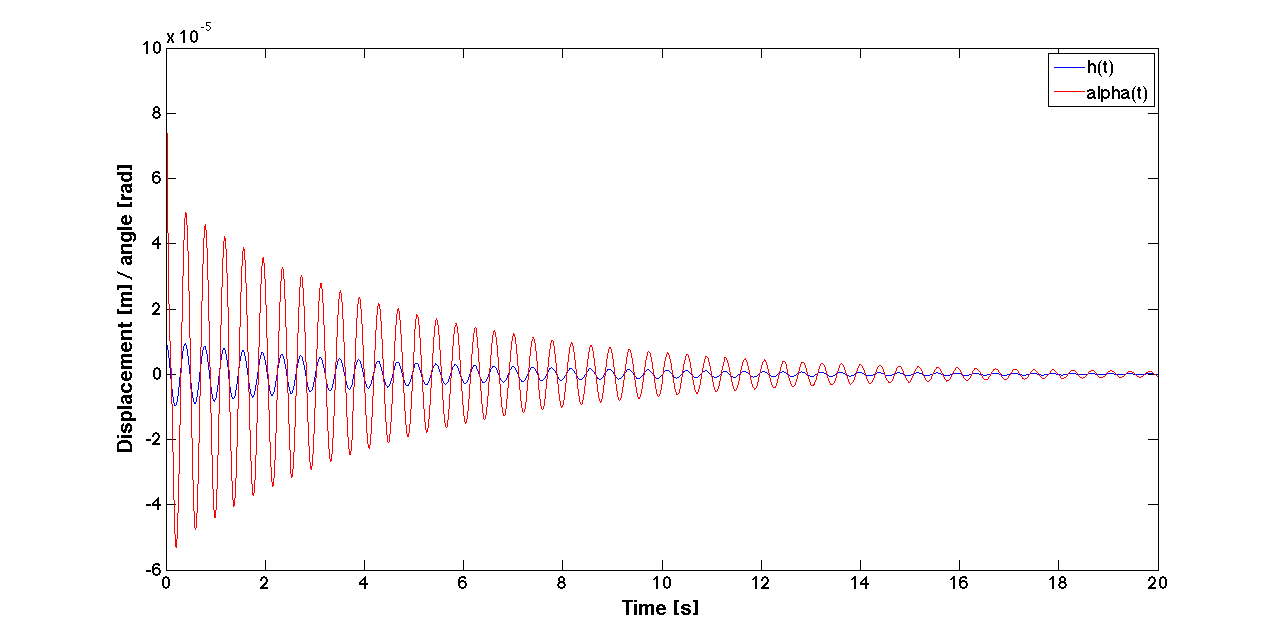
\includegraphics[width=1.0\textwidth]{k20attract.png}
\caption{\label{fig:k20attract} A plot of $h$ and $\alpha$ against $t$ showing how the system returns to its equilibrium at $U=10$ when a miniscule perturbation is applied.  }
\end{figure}

\noindent The first stability state that the equilibrium has is as an attractor (as shown in Figure \ref{fig:k20attract}). This only occurs incredibly close to the equilibrium, when the initial perturbation is very small. 

\begin{figure}[H]
\centering
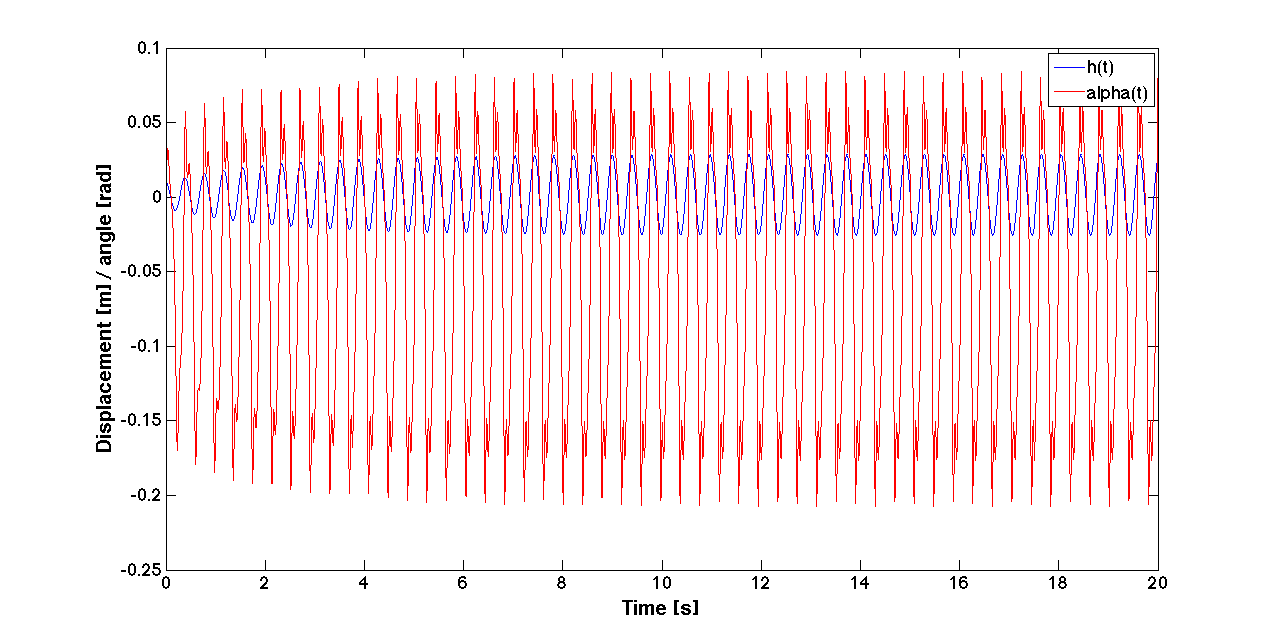
\includegraphics[width=1.0\textwidth]{k20repel.png}
\caption{\label{fig:k20repel} A plot of $h$ and $\alpha$ against $t$ showing how the system response becomes a limit cycle at $U=10$ when a small perturbation is applied.  }
\end{figure}

\noindent The next stability state of the equilibrium is a repeller. This is when a small perturbation is used, and the system moves to a limit cycle. The bifurcation occurs between $U=14$ and $U = 15$ again, and then the stability becomes a repeller, and a limit cycle is created, as can be seen in Figure \ref{fig:k20repel}.

\subsubsection{Changes in the Bifurcation}
%Difference in bifurcation?

As the equilibrium has stayed the same, so too has the bifurcation point; it is still between $U = 14$ and $U = 15$. The difference is that the Hopf bifurcation has turned from a supercritical bifurcation in to a subcritical bifurcation. This is shown from Figure \ref{fig:k20repel}, where a limit cycle can be seen at $U = 10$, before the bifurcation. This is in direct contrast to the original system, where the limit cycle occured only after the bifurcation. A limit cycle for this system also occurs after the bifurcation, but this is due to the fact that, because a real system is being analysed, the parameters are unable to tend to infinity as would happen in an ideal subcritical bifurcation. Thus, the limit cycle after the bifurcation is created. 

\subsection{Increasing $k_{\alpha_{1}}$ further}

This section deals with what happens when $k_{\alpha_{1}}$ is increased above 20. 

\subsubsection{Equilibria}

As $k_{\alpha_{1}}$ increases to above 20, the complex equilibria from Section \ref{sec:equilibria} become real. This means that the system now has three equilibria for $k_{\alpha_{1}} > 20$.

\subsubsection{The New Jacobian}
%Describe what happens when this value is changes
%calculate new Jacobian
As the Jacobian found in Section \ref{sec:jacobian} is only valid for the trivial solution, the first step for finding solutions that could relate to other equilibria is to find the Jacobian that takes the nonlinear terms in to account. 

\begin{equation}
\label{eqn:statespace}
\begin{array}{lll}
q_{1} & = & {q} \\ 
q_{2} & = & \dot{q} \\
q_{2} & = & \dot{q_{1}}\\
\dot{q_{2}} & = & -CM^{-1}q_{2}-KM^{-1}q_{1}+N(q)M^{-1}\\
\end{array}
\end{equation}\\


\noindent This is done by first putting the system in to state space form, as can be seen from Equation \ref{eqn:statespace}. Once the system is in state space form, the Jacobian can be found. This is calculated using the partial derivatives of the state space equations. The results of this are shown in Equation \ref{eqn:newjacobian}.

\begin{equation} \label{eqn:newjacobian}
\begin{pmatrix}
  \underline{\underline{0}} & \underline{\underline{I}} \\ \\
  -\underline{\underline{M}}^{-1} \underline{\underline{K}} - \underline{\underline{M}}^{-1} \nabla N & -\underline{\underline{M}}^{-1} \underline{\underline{C}}
  \end{pmatrix}
  \end{equation} \\
  
\noindent This Jacobian is a four-by-four matrix, as it is with respect to two variables, $h$ and $\alpha$, where $\nabla N$ is the Jacobian of N. This is added because the new Jacobian has to be affected by nonlinear terms, and this Jacobian gives the same results as the one used in section \ref{sec:jacobian} for when $\alpha$ and $h$ are 0. 



%See what happens as U increases
%complex conjugate equilibrium become real
%what is the stability of the equilibrium?